\documentclass{standalone}
\usepackage{xcolor}
\usepackage{verbatim}
\usepackage[T1]{fontenc}
\usepackage{graphics}
\usepackage{hyperref}
\newcommand{\code}[1]{\texttt{#1}}
\newcommand{\R}{R}
\newcommand{\pkg}[1]{#1}
\newcommand{\CRANpkg}[1]{\pkg{#1}}%
\newcommand{\BIOpkg}[1]{\pkg{#1}}
\usepackage{amsmath,amssymb,array}
\usepackage{booktabs}
\usepackage{tikz}
\usetikzlibrary{arrows,positioning,shapes.geometric}
\usetikzlibrary{calc}
\usepackage[normalem]{ulem}
\usepackage{mathtools}
\usepackage{graphicx}
\usepackage{makecell}
\usepackage{bm}

\begin{document}
\nopagecolor
    \centering
    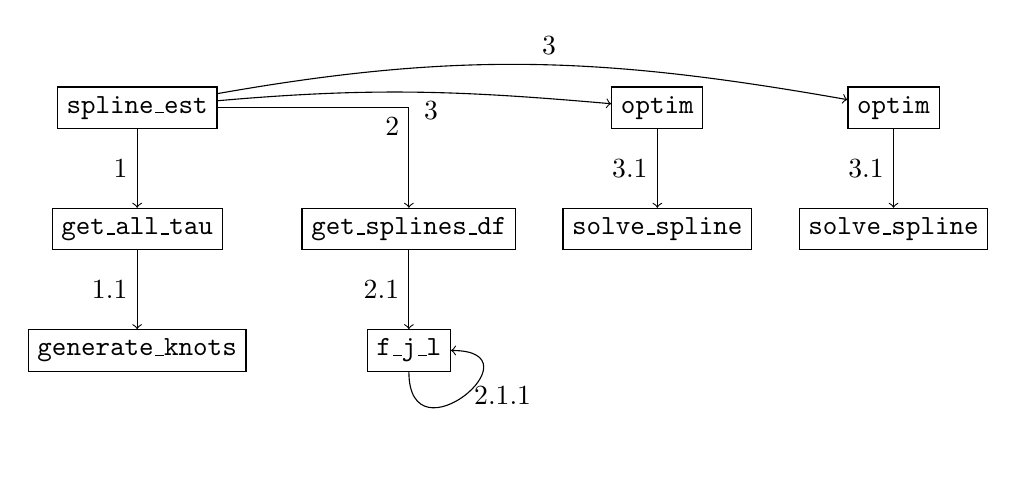
\begin{tikzpicture}
        \tikzstyle{block} = {draw, rectangle, align=center, minimum width=2cm,minimum height=1cm}
        \tikzstyle{line} = [draw, -latex'],
        \node [block,align=center]  (spline_est) {{\ttfamily spline\_est}};
        % Step 1
        \node [block,align=center , below = 1cm of spline_est]  (get_taus) {{\ttfamily get\_all\_tau}};
        \node [block,align=center , below = 1cm of get_taus]  (generate_knots) {{\ttfamily generate\_knots}};
        % Step 2
        \node [block,align=center , right = of get_taus]  (splines_df) {{\ttfamily get\_splines\_df}};
        \node [block,align=center , below = 1cm of splines_df] (adjusted_spline) {{\ttfamily f\_j\_l}};
        % Step 3
        \node [block,align=center , right = 5cm of spline_est]  (optim1) {{\ttfamily optim}};
        \node [block,align=center , right = 8cm of spline_est]  (optim2) {{\ttfamily optim}};
        \node [block,align=center , below = 1cm of optim1]  (solve_spline1) {{\ttfamily solve\_spline}};
        \node [block,align=center , below = 1cm of optim2]  (solve_spline2) {{\ttfamily solve\_spline}};
        % Connections
        \draw [->] (spline_est) -- (get_taus) node[midway, left] {1};
        \draw [->] (get_taus) -- (generate_knots) node[midway, left] {1.1};
        \draw [->] (spline_est) -| (splines_df) node[midway, below left] {2};
        \draw [->] (splines_df) -- (adjusted_spline) node[midway, left] {2.1};
        \draw [->] (adjusted_spline) to [out=270, in=0, looseness=5] node[right] {2.1.1} (adjusted_spline);
        \draw [->] (spline_est) to [out=5, in=175] node[below right] {3} (optim1);
        \draw [->] (spline_est) to [out=10, in=170] node[above right] {3} (optim2);
        \draw [->] (optim1) -- (solve_spline1) node[midway, left] {3.1};
        \draw [->] (optim2) -- (solve_spline2) node[midway, left] {3.1};
    \end{tikzpicture}
\end{document}
